\chapter{Testing \& Evaluation}
	
	\label{sec:testing}
	
	As the system was built, the individual parts were unit-tested extensively
	before integration into the rest of the system. Integration tests were then
	performed followed finally by a series of full system tests. This strategy
	made testing was a continuous process throughout the implementation and
	identified bugs early.
	
	In this chapter the tests carried out during development are described along
	with an evaluation of the results. Each section describes the tests a major
	component of the system was subjected to concluding with an evaluation of the
	system's overall performance.
	
	\section{Electronics}
		
		The major components of the electronics were prototyped and tested on a
		breadboard with the use of a multimeter. The higher power components, such
		as the heaters and motors, were initially disconnected or tested with
		low-power test loads until the circuit was deemed to be correct. Once
		connected, these components were then tested under operational loads with
		careful supervision to ensure that they functioned correctly and that the
		current flowing through each part of the circuit was as expected. The tested
		circuit designs were then soldered together on circuit boards where the
		connections were first tested for continuity and checked for short circuits
		before performing integration tests on the system.
		
		Overall the electronics performed well and no problems caused by electrical
		noise generated when switching high-power loads were observed. The parts of
		the system which were found to exhibit unexpected behaviour are outlined in
		the following subsections.
		
		\subsection{MOSFETs}
			
			The MOSFETs were able to switch on the heaters and bring the system from
			room temperature to operating temperature within 10 minutes, matching the
			performance of the previous system as expected.
			
			After an extended period of being powered on, the MOSFETs became hot
			running at around 50\dC. The data sheet for the IRLU8729PbF MOSFETs states
			that the operating temperature range is from $-55\dC{}$ to 175\dC{} and so
			this temperature is safely within operational limits.
		
		\subsection{End-stops}
			
			Printed plastic paddles were originally planned as the triggers for use
			with the end-stops. Unfortunately, acrylonitrile butadiene styrene (ABS)
			plastic used by the Makerbot is transparent to the infra-red wavelengths
			used by the opto-interrupters and so this material is unsuitable. The
			design was changed to instead use wooden craft `lollipop sticks' which fit
			into pre-cut slots in the Makerbot and easily trigger the
			opto-interrupters.
		
		\subsection{ATX PSU}
			
			Some ATX PSUs require a certain load on all provided voltages in order to
			power up properly \cite{reprapatx}. While a large load is drawn on the 12V
			line by the heaters and motors, the 5V line only powers the Mbed which
			draws little power. The result of this is that the 12V line attached to
			the heaters only provided 9V and so could not warm up to the required
			temperature.
			
			A resistor can be added to the 5V line to draw extra current and fully
			power up the PSU \cite{reprapatx}. Due to time constraints an alternative
			PSU was used which did not feature this behaviour rather than modifying
			the circuit. With the new PSU, all voltages met their specified
			requirements.
	
	\section{FreeRTOS}
		
		The availability of the FreeRTOS port made it extremely easy to integrate
		into the project. FreeRTOS itself provided the right balance of features and
		performance for the project. The operating system did not place restrictions
		on the use of low-level system registers and simply provided preemptive
		multitasking and some atomic operations as required.
		
		The operating system was initially tested for timing accuracy using a
		frequency probe attached to an I/O pin toggled by a simple demonstration
		program to ensure the system was behaving as expected. This test yielded a
		mismatch from the expected frequency which was found to be an incorrect
		definition of the system clock speed in a FreeRTOS header file. Once fixed
		the system ran as expected running the included demo and test programs as
		defined. No further issues were found during the course of the project.
	
	\section{\uIP{} \& Networking}
		
		Various tests were conducted on the \uIP{} stack during the project,
		concentrating on performance and correctness of the features used. This
		section discusses these tests and concludes with an evaluation of \uIP{}'s
		suitability for the project.
		
		\label{sec:udpPerformance}
		
		Wireshark was used to monitor the packets sent between the Mbed and computer
		where it became apparent that every packet from the Mbed was being
		duplicated. After ruling out network problems as the cause, the bug was
		traced down to the Ethernet driver provided by the demo. The driver
		duplicated every packet sent to the network (including IMCP Ping Requests,
		figure \ref{fig:ping}). As well as wasting bandwidth, if a TCP packet
		acknowledgement (ACK) from the Mbed was to be delayed in the network,
		retransmission will result in four duplicate ACK packets. This causes the
		sending computer to retransmit and incorrectly adjust its expectations of
		the network connection when the packets are eventually received
		\cite{duplicateack}. This behaviour is one factor that can prevent TCP flow
		control from functioning correctly.
		
		\begin{figure}
			\begin{verbatim}
				$ ping 192.168.3.100
				PING 192.168.3.100 (192.168.3.100) 56(84) bytes of data.
				64 bytes from 192.168.3.100: icmp_req=1 ttl=64 time=0.364 ms
				64 bytes from 192.168.3.100: icmp_req=1 ttl=64 time=0.385 ms (DUP!)
				64 bytes from 192.168.3.100: icmp_req=2 ttl=64 time=0.175 ms
				64 bytes from 192.168.3.100: icmp_req=2 ttl=64 time=0.195 ms (DUP!)
				64 bytes from 192.168.3.100: icmp_req=3 ttl=64 time=0.195 ms
				64 bytes from 192.168.3.100: icmp_req=3 ttl=64 time=0.212 ms (DUP!)
				64 bytes from 192.168.3.100: icmp_req=4 ttl=64 time=0.179 ms
				64 bytes from 192.168.3.100: icmp_req=4 ttl=64 time=0.195 ms (DUP!)
				^C
				--- 192.168.3.100 ping statistics ---
				4 packets transmitted, 4 received, +4 duplicates, 0% packet loss, time 3000ms
				rtt min/avg/max/mdev = 0.175/0.237/0.385/0.081 ms
			\end{verbatim}
			\caption{Ping responses being duplicated by the \uIP{} driver}
			\label{fig:ping}
		\end{figure}
		
		The packet duplication behaviour is often added to \uIP{} implementations to
		work around problems caused by \uIP{} only allowing one packet to be sent at
		a time \cite{allpacketsdup}. Modern systems (such as Windows and Linux) will
		allow several packets to arrive before acknowledging them all at once,
		saving bandwidth reducing the effect of network latency. This delays the
		transmission of the next packet by \uIP{} as it waits for the ACK. By
		duplicating each packet, the receiving computer is forced to immediately
		send an ACK as, from receiver's perspective, a duplicate packet may indicate
		that the original packet was delayed in the network and the sender did not
		receive an ACK in time in this case because the receiver had never sent it.
		As a result the receiver sends the ACK immediately allowing \uIP{} to send
		the next packet.
		
		Though this wastes bandwidth it reduces the wait between each packet being
		sent and in practice dramatically increases the bandwidth available when
		sending data from the Mbed to the computer. Disabling this work-around means
		sending multiple-packet bursts of data to a computer is more time consuming
		but removes a barrier to flow control being used successfully. The only data
		sent from the Mbed are status responses which are small enough (around 30
		bytes) to fit in a single packet. Disabling packet duplication, in favour of
		removing a barrier to proper flow control, is a good trade off.
		
		\label{sec:tcpProblem}
		
		Unfortunately, problems with flow control persisted with no improvement
		after disabling packet duplication. With the duplicate packets removed, the
		traffic became clearer. To enable flow control, TCP sends a window size with
		each packet representing the amount of data the receiver is able to receive.
		\uIP{} reports a constant window size until the method \verb|uip_stop()| is
		called when the window size is set to zero and any further packets received
		are discarded. The zero window message is resent until \verb|uip_restart()|
		is called and the old window size is restored. A packet is then sent to the
		computer to request data transfer to continue.
		
		To test this mechanism, a program was written which produced a long sequence
		of small movement G-code instructions. This causes the buffer to initially
		fill up and then be constantly kept topped up by the computer while being
		restrained by flow control. The actual behaviour of the connection (shown in
		figure \ref{fig:uIPFlowControl}) shows the buffer is initially filled (the
		first spike) but then the sender waits an exponentially growing period until
		it starts filling the buffer again regardless of when the window size is
		made non-zero.
		
		\begin{figure}
			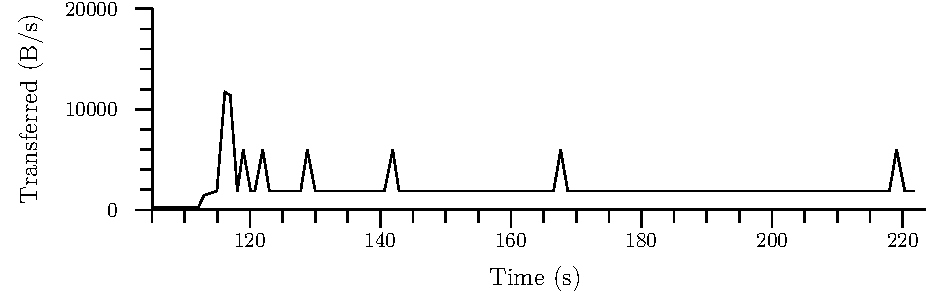
\includegraphics[width=1\textwidth]{diagrams/uIPFlowControl.pdf}
			\caption{Exponential back-off by computer when \uIP{} flow-control used}
			\label{fig:uIPFlowControl}
		\end{figure}
		
		By inspecting the packets sent and received, the window size is always
		obeyed by the computer but the packet announcing the window size becoming
		non-zero appears to be ignored as transmission is not immediately resumed.
		Wireshark's protocol checker did not report any errors and comparison with
		the known-working implementation of TCP flow control in Linux did not reveal
		any obvious differences. Unfortunately further study did not yield a
		diagnosis for the problem. Due to the time constraints imposed by the
		project TCP had to be dropped for G-code transmission in the project.
	
	\section{Temperature Readings}
		
		The temperature readings depended on correct values being read from the
		analog inputs and on correct calculation of the temperature based on these
		readings. Consistency of readings is important, reading temperatures close
		to the actual value, however, is relatively unimportant. This is because the
		temperature is fairly uneven within the heated components of the printer and
		so it is difficult to define a `correct' reading. The actual temperature
		values used during printing are calibrated manually and so the absolute
		temperature in \dC{} is not significant.
		
		To test analog input, a selection of resistors with known values within the
		range of values the thermistor could exhibit were tested. As well as
		breadboard testing, the test was repeated on the final circuit board as the
		screw terminal used to connect the thermistors could also be used to connect
		a test resistor directly.
		
		When converted to a resistance using (\ref{equ:potdiv}), the values read
		were found to be within $\pm2\%$ of the resistor value as read by a
		multimeter (a difference which is accounted for by the fact that a second
		resistor with a $\pm5\%$ tolerance is used in the potential divider).
		
		To test that temperatures were being correctly calculated, an infra-red
		thermometer (figure \ref{fig:thermometer}) was used to take reference
		temperature readings from the extruder and platform. The heaters were turned
		on and readings were taken every minute as the extruder and platform heated
		up and then every five minutes for half an hour as it cooled down.  The
		tests were repeated multiple times alongside other experiments, each time
		with similar results, to ensure consistency. These values were then compared
		against the value calculated using (\ref{equ:steinhart}). 
		
		The radius of the area measured by the thermometer becomes larger as it is
		moved further away from the target. Because the temperature across the
		platform and extruder vary greatly depending on location, the thermometer
		was placed close to the centre of the extruder nozzle and the centre of the
		build platform where the thermistors reside.
		
		\begin{figure}
			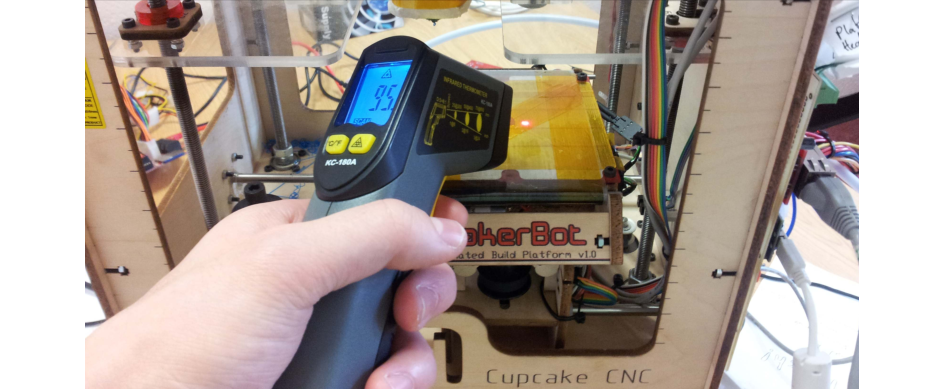
\includegraphics[width=1\textwidth]{diagrams/thermometer.pdf}
			\caption{Checking platform temperatures using an infra-red thermometer}
			\label{fig:thermometer}
		\end{figure}
		
		The temperatures recorded for the extruder were within $\pm1\dC$ below
		100\dC{} but rose to around $+8\pm1\dC$ around 220\dC{} (normal operating
		temperature).
		
		The platform temperatures were initially incorrect by $\pm10\dC$ or more.
		This was caused by a simple connection error. Once the problem was
		corrected, readings followed a similar pattern to the extruder (up to the
		125\dC{} the platform is designed to operate at).
		
		The results above represent adequate performance for the task of maintaining
		a desired temperature and also show that the temperatures read are close to
		their real values such that an operator can safely tell from a temperature
		reading that the device is unsafe to touch. The error at high temperatures
		may be a result of not being able to use the thermometer to measure the
		internal parts of the extruder where it is hottest.
	
	\section{PID Control}
		
		\label{sec:pidtraning}
		
		The PID controller has three constants ($K_p$, $K_i$ and $K_d$) which must
		be manually tuned to yield sensible system performance. An optimal system
		has oscillations in temperature that are as small as possible.
		
		PID controller tuning is a non-trivial problem for which automated solutions
		are either highly specialised or unavailable. Heuristics exist such as The
		Ziegler-Nichols method for selecting good values which work in many cases
		and require human interpretation \cite{ziegler}.
		
		The Makerbot wiki suggests values (given in table \ref{tab:makerbotpid})
		which yield adequate performance on many printers \cite{makerbotpid}. After
		selecting these values the printer's performance was monitored both while
		idle and during printing and the size of the oscillations were measured.
		Performance was similar in both states (with the exception of a temperature
		jump in platform temperature at the start of printing caused by molten
		plastic being extruded on top of the thermistor). Oscillations were
		$\pm2\dC$ for the extruder and platform. Due to time constraints, further
		improvements in tuning could not be achieved. Though this is greater than
		the $\pm1\dC$ recommended, print quality was not adversely affected.
		
		\begin{table}
			\centering
			\begin{tabular}{l l l}
				\toprule
				Constant & Extruder Value & Platform Value \\
				\midrule
				$K_p$    & $5.143$        & $7.0  $  \\
				$K_i$    & $0.0612$       & $0.342$ \\
				$K_d$    & $108.0$        & $36.0 $  \\
				\bottomrule
			\end{tabular}
			
			\caption{Generic PID controller constants for a Makerbot
			         \cite{makerbotpid}}
			\label{tab:makerbotpid}
		\end{table}
	
	\section{Stepper Control}
		
		The amount of plastic deposited at a given point during a print is dependent
		on the rate at which the plastic is extruded and also the rate at which the
		platform moves. The accuracy of the timing (combined with the mechanical
		properties of the machine) determines the platform's rate of movement and
		thus the print quality.
		
		The stepper control system consists of code for producing accurately timed
		steps and code for coherently moving the stepper motors. These two parts
		were tested separately as described in the following subsections.
		
		\subsection{Timing}
			
			To ensure timing accuracy, the three stepper signals were driven at a
			combination of frequencies with a frequency probe attached to the step
			pin. These tests were generated initially using a program on the
			microcontroller (so that the system was not under any load) and then using
			G-code sent over the network interface while other requests were being
			made (to place the system under reasonable load).
			
			The frequencies measured were exact to within the accuracy of the probe
			(four significant figures) for all tests.
			
		
		\subsection{Stepping}
			
			To test that steps happened coherently, with sequences of steps correctly
			spaced apart, the system was connected to the printer and circles were
			plotted. The circles are made up of short, continuous line segments where
			the relationship between the movements on each axis varies. Once again,
			the test was initially conducted using a test program running on the Mbed
			and then by G-code sent over the network. The number of segments the
			circle was divided into was increased from $30$ to $3,000$ and the speed
			set to $330\mm/\minute$ and $3300\mm/\minute$ to test slow and fast
			movements.
			
			The performance of the system was measured by visual inspection of the
			movement and circles plotted by attaching a pen to the extruder. The time
			taken the plot the circles was also measured using a timer on the Mbed to
			see if the processing overhead between each segment caused significant
			drift. Above around $100$ segments the circles drawn appeared smooth and
			at low and high speeds the overhead after 20 circles had been plotted at
			each speed and resolution was less than the $1\ms$ resolution of the
			timer. Finally, to ensure that steps were not missed, the system was moved
			to a known point between tests and this did not drift after all tests had
			completed.
	
	\section{End-stops}
		
		The endstops were tested under various lighting conditions to observe the
		effect of external lighting on the opto-interrupters. The following
		lightings conditions were tested:
		\begin{itemize}
			\item Ambient strip lighting
			\item Ambient halogen lighting
			\item Ambient incandescent lighting
			\item Ambient natural light
			\item Direct halogen lighting
			\item Direct incandescent lighting
			\item Darkened room
		\end{itemize}
		
		Testing consisted of blocking each opto-interrupter by moving the printer
		axes so that the end-stop is triggered and observing the digital value read
		by the Mbed and the state of the debugging LED. Under all but the direct
		lighting conditions the correct value was read and the debugging LEDs were
		either completely off or completely on. Under direct lighting, especially
		incandescent lighting, the state read by the Mbed for some end-stops became
		stuck due to external light shining into the opto-interrupters. In these cases
		the debugging LEDs did not become completely `off' indicating that the
		opto-interrupter was being only partially triggered.
		
		Though these results suggest that the end-stops cannot be used under direct
		lighting from halogen or incandescent bulbs, the system was found to perform
		well outside these conditions. Although not tested due to unfavourable
		weather conditions, direct natural light may also have caused similar
		problems. While these restrictions are unfortunate, they are not
		unreasonable and still allow the system to be used in practice.
	
	\section{Buffer Utilisation}
		
		To ensure that the printer pipeline did not stall during print jobs, the
		G-code and low-level command buffers were monitored during the execution of
		various test jobs. If buffer underruns occurred or poor buffer utilisation
		was observed, it could indicate a performance issue in the G-code
		interpreter, network interface or their interaction with the operating
		system.
		
		The utilisation of each buffer along with a counter for the number of
		underruns experienced by the command-buffer were logged while various G-code
		files were sent to the printer. Most testing was carried out during the
		system testing phase but the following synthetic tests were also used.
		
		\begin{description}
			
			\item[Circle plotting with low detail] This test ensured that, given a
			sequence of slow G-code instructions, the printer keeps all buffers
			reasonably full and that the network interface can cope with small,
			infrequent bursts of data.
			
			\item[Circle plotting with high detail] This test ensures that, given a
			constant sequence of fast G-code instructions, the printer keeps all
			buffers reasonably full and that no underruns occur during busy periods.
			
			\item[Circle plotting with high detail and pauses] This test ensures that
			given a sequence of fast G-code instructions separated by pauses (where
			the buffers filled and the network interface paused) the transmission can
			quickly restart after the pause.
			
		\end{description}
		
		In all tests the buffer levels were generally above half full in the worst
		case. In a small number of instances the underrun counter was triggered but
		no effect on the printer was observed. These underruns may have been the
		result of FreeRTOS not allocating enough resources to the G-code interpreter
		until the low-level command buffer emptied (but while the G-code buffer was
		still full). Once the G-code interpreter was allowed to execute, printing
		would have continued immediately resulting in the unobservable pauses
		observed.
	
	\section{System Testing}
		
		The system was tested as a whole to assess its performance in both printing
		synthetic benchmarks as well as printing real-world objects. These tests
		also aided in calibration of the G-code generator (Skeinforge). The
		synthetic tests allow the printer's performance to be objectively measured
		while real objects show the real-world performance of the printer in its
		intended application.
		
		\subsection{Synthetic Tests}
			
			As a simple test of using all of the printer's components coherently, the
			circle plotting test was modified to produce spirals and the heaters and
			extruder enabled. Figure \ref{fig:syntheticTests} shows samples of the
			output of these tests:
			\begin{description}
				
				\item[(A)] The extruder was moved at a safe distance from the platform
				to ensure that all components move coherently but without the risk of
				the extruder colliding with the platform or blocking the nozzle of the
				extruder.
				
				\item[(B)] As in (A) but the extruder is moved closer to the platform to
				test that the system can safely operate close to the platform and that
				the plastic adheres properly (and then is properly detached when
				ejected).
				
				\item[(C)] A larger spiral was printed to test that the plastic adheres
				closer to the (colder) edges of the platform and that warping due to
				temperature changes during the print, does not cause problems.
				
				\item[(D)] The winding of the spiral was tightened to test that the
				plastic adheres to itself and the platform and that warping does not
				cause the print to fail. Figure \ref{fig:looseSpiral} shows a print
				where the spiral was printed too loosely and it did not adhere to
				itself.
				
			\end{description}
			
			\begin{figure}
				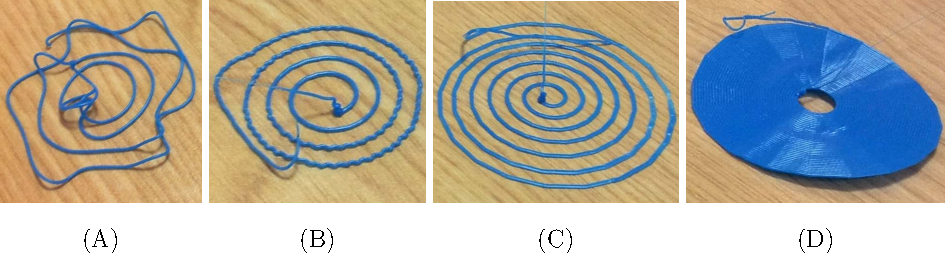
\includegraphics[width=1\textwidth]{diagrams/syntheticTests.pdf}
				\caption{Synthetic 3D printer tests for basic calibration}
				\label{fig:syntheticTests}
			\end{figure}
			
			\begin{figure}
				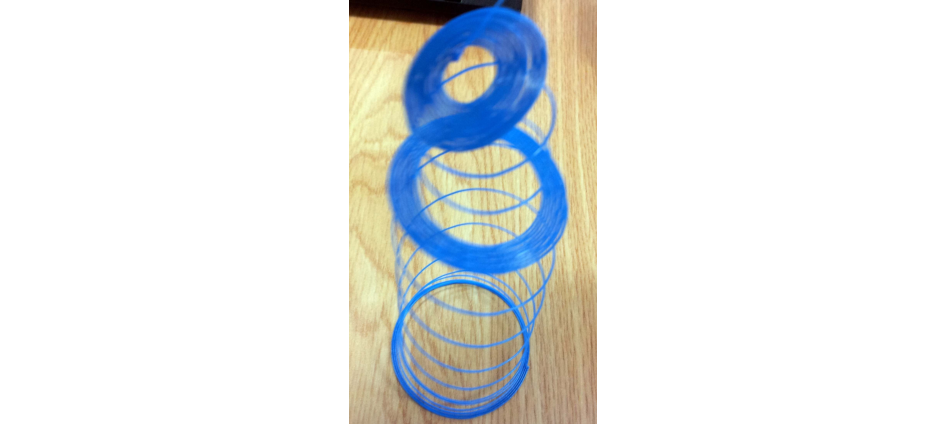
\includegraphics[width=1\textwidth]{diagrams/looseSpiral.pdf}
				\caption{Bad print of the test in figure \ref{fig:syntheticTests}(D)}
				\label{fig:looseSpiral}
			\end{figure}
			
			These prints were repeated, varying the platform temperature, Z-axis
			position (height) and the tightness of the spiral until the tests
			performed as described above. These tests ensure that the printer is
			capable of operating all its major components coherently in order to
			produce printed object.
			
			To test the system with G-code generated by Skeinforge, a simple 3D model
			of a cuboid (Figure \ref{fig:testCubes} (A)) was printed. This print
			yields a cuboid of known dimensions and used to check calibration settings
			for Skeinforge and assess the printer's performance. The cuboid was
			initially printed on top of a thick `raft' of plastic (used to ensure an
			even printing surface) and then separated using a chisel.
			
			The dimensions of the cuboids were checked using a pair of digital
			callipers (figure \ref{fig:calipers}) to ensure that the printed object is
			of the correct size. The Makerbot wiki claims that $0.1\mm$ resolution is
			possible on a correctly tuned machine and this requirement was met by most
			of the printed cuboids \cite{makerbotfaq}. In a small number of cases, the
			Z-axis of the printer did not move the required amount due to the
			mechanism jamming, a known problem with the Makerbot design
			\cite{zaxisissue}. As a result, these prints were of the incorrect height
			but were otherwise correct and the problems not attributed to the
			firmware.
			
			\begin{figure}
				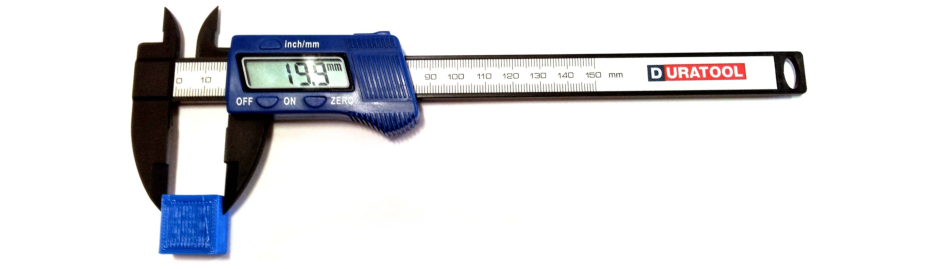
\includegraphics[width=1\textwidth]{diagrams/calipers.pdf}
				\caption{Digital callipers being used to measure test cuboids}
				\label{fig:calipers}
			\end{figure}
			
			\begin{figure}
				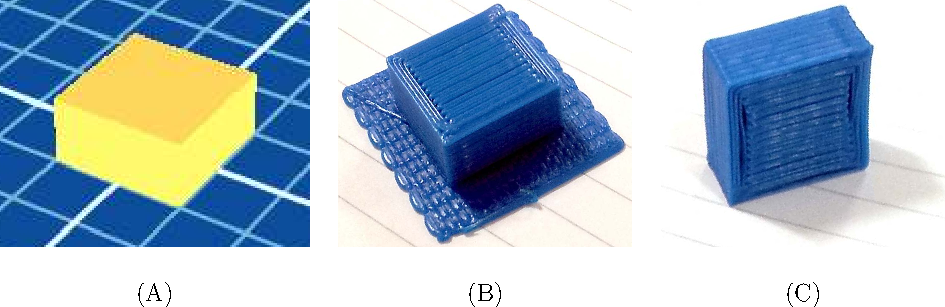
\includegraphics[width=1\textwidth]{diagrams/testCubes.pdf}
				\caption{Test cuboid model (A) print from Skeinforge G-code before raft
				         removal (B) and after raft removal (C)}
				\label{fig:testCubes}
			\end{figure}
			
		
		\subsection{Test Objects}
			
			To test the printer's ability to produce useful objects, various objects
			were printed including objects with moving parts or near the
			print size limits of the printer. These tests check the system's ability
			to deal with large and complex loads. A selection of printed test objects
			is provided in Appendix \ref{sec:examplePrints}.
			
			\subsubsection{Detailed Prints}
				
				Prints with detailed areas were used to test that the system could
				process the larger density of G-code at the required rate and also to
				ensure that steps were not missed during printing.
				
				For example, figure \ref{fig:vase} shows a vase which yields very short
				line segments while printing the corners of the shape. The previous
				electronics would not be able to process this design fast enough and
				would skip instructions causing steps to be missed. With the new
				electronics no buffer underruns or printing problems occurred during a
				run featuring a large version (shown) and a smaller version containing
				finer detail.
				
				\begin{figure}
					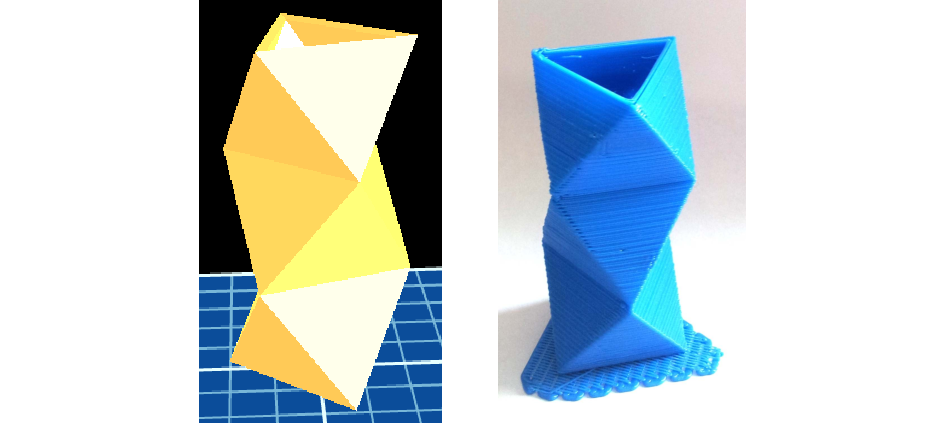
\includegraphics[width=1\textwidth]{diagrams/vase.pdf}
					\caption{3D printed vase with detailed corners}
					\label{fig:vase}
				\end{figure}
				
				Figure \ref{fig:handle} shows an object which has a small cylindrical
				handle printed with the old and new electronics. With the old system,
				the G-code was not processed fast enough resulting in the printer
				stalling and depositing extra plastic. The new system was able to
				process the same amount of G-code without stalling.
				
				\begin{figure}
					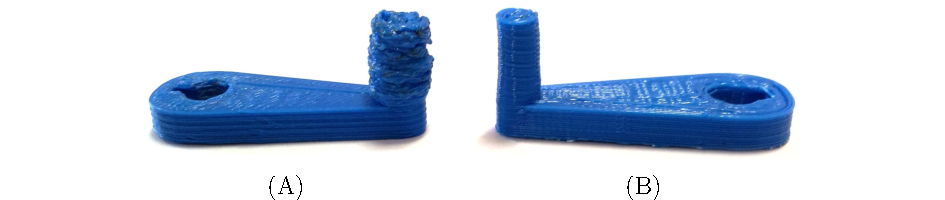
\includegraphics[width=1\textwidth]{diagrams/handle.pdf}
					\caption[3D printed Z-axis handle comparison]{3D printed Z-axis handle
					comparison of old (A) and new (B) electronics}
					\label{fig:handle}
				\end{figure}
				
				Figure \ref{fig:herringbone} shows a pair of herringbone gears printed
				with the old and new electronics. (A) and (B) show how the new system is
				able to produce rounder circles due to better timing accuracy. (C) and
				(D) show the effect of improved timing accuracy on the teeth of the
				gears.
				
				\begin{figure}
					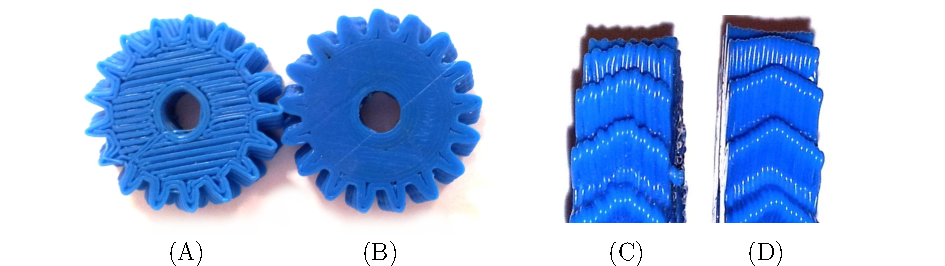
\includegraphics[width=1\textwidth]{diagrams/herringbone.pdf}
					\caption[3D printed herringbone gear comparison]{3D printed
					herringbone gear comparison of old (A) \& (C), and new (B) \& (D)
					electronics}
					\label{fig:herringbone}
				\end{figure}
			
			\subsubsection{Large Prints}
				
				Large prints stress the printer and electronics for long periods and can
				reveal missed motor steps or instructions. The previous system had
				frequent issues printing large test objects due to skipped instructions
				or steps and is a particular area for improvement.
				
				Of the large objects printed, only one failed to print (figure
				\ref{fig:failedPrint}). This was due to the object warping (A) and then
				becoming detached from the platform during the print causing the tip of
				the extruder to rip the object off the platform (B). Unevenness in the
				temperature of the object during printing is the cause of this
				distortion. This is partially caused by unevenness in the temperature of
				the build platform. Unfortunately, this is a problem with the printer's
				design which is not addressed in this project.
				
				\begin{figure}
					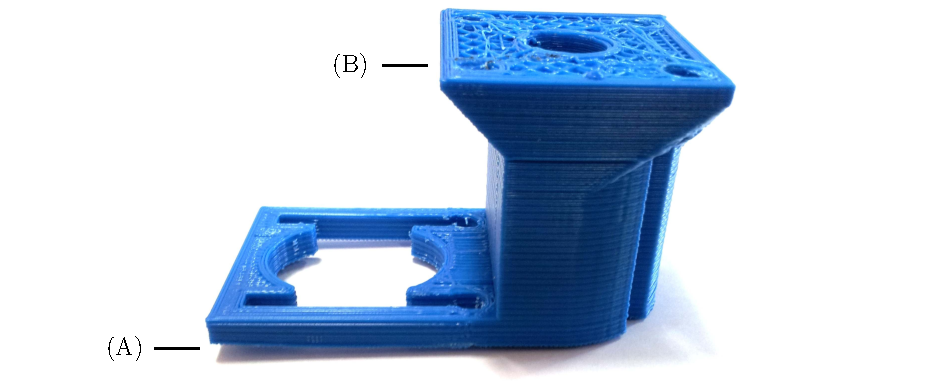
\includegraphics[width=1\textwidth]{diagrams/failedPrint.pdf}
					\caption{Failed large print showing warping (A) and a collision with
					         the extruder (B)}
					\label{fig:failedPrint}
				\end{figure}
			
			\subsubsection{Raftless Printing}
				
				Though the first prints were completed on top of a raft, it was later
				disabled. This reduced print time, improved print quality and allowed
				intricate designs such as combs to be printed where removal of a raft
				would damage the design (figure \ref{fig:comb}).
				
				\begin{figure}
					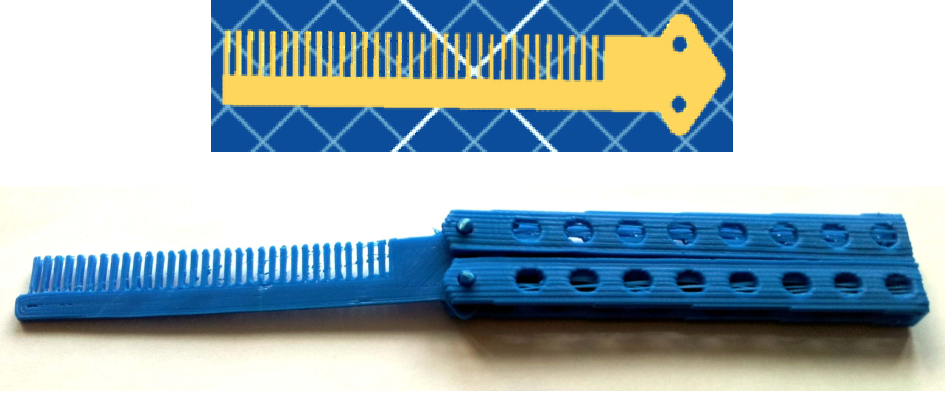
\includegraphics[width=1\textwidth]{diagrams/comb.pdf}
					\caption{Folding `butterfly comb', printed without a raft}
					\label{fig:comb}
				\end{figure}
				
				Many objects were reprinted using raftless printing and performance was
				generally similar with the exception of larger designs. These
				experienced greater warping without the support of the raft and thus
				were more prone to failure due to the extruder hitting the object.
